\documentclass{beamer}

\usepackage{graphicx}
\usepackage{enumerate}

\title % (optional, only for long titles)
{Dynamical Systems as Gaussian Process \newline Prior  Distributions}
\author{Nathan Wycoff}
\institute[Virginia Tech] % (optional)
{
	Virginia Tech
}
\date{December 6, 2016}
\subject{Machine Learning}

\AtBeginSection[]
{
	\begin{frame}
		\frametitle{Table of Contents}
		\tableofcontents[currentsection]
	\end{frame}
}

\begin{document}
	\frame{\titlepage}
	
	\begin{frame}
		\frametitle{Table of Contents}
		\tableofcontents
	\end{frame}
	
	\section[Section]{Motivation}
	
	\begin{frame}
		\frametitle{Mathematical Spatial Models}
		
		\begin{itemize}
			\item Separate suite of methods for spatial analysis.
			\item Makes use of subject matter theory based on partial differential equation systems.
			\item Ex: Murray, \textit{Mathematical Biology II: Spatial and Biomedial Applications}
		\end{itemize}
		
		\vspace{1em}
		
		How can different kinds of spatial analysis merge?

		
		
	\end{frame}
	
	\begin{frame}
		\frametitle{Dynamical Systems}
		
		Description of something over time.
		
		
		\vspace{2em}
		
		Examples:
		
		\begin{itemize}
			\item Standard Equation:
			
			$$y(t) = f(t)$$
			
			\item Differential Equation:
			
			$$\frac{\partial^i y(t)}{\partial t^i} = f(\frac{\partial^i y(t)}{\partial t^i}, \frac{\partial^i y(t)}{\partial x_j^i})$$
			
			\item Difference Equation:
			
			$$y_{t+1, j} = f(y_{t-i,j+k})$$
			
		\end{itemize}
		
		
		
	\end{frame}
	
	
	
	\begin{frame}
		\frametitle{Theme}
		
		\begin{itemize}
			\item GP kernels as priors on functions
			\item Informative kernels
		\end{itemize}
		
		\vspace{1em}
		
		Central Question
		
		Can we use a dynamical system as prior information for a GP through a kernel?
		
		Importance:
		
		\vspace{1em}
		
		\begin{itemize}
			\item Include information about system dynamics
			\item Separate signal from noise
		\end{itemize}
	\end{frame}
	
	\section[Section]{Methods}
	
	\begin{frame}
		\frametitle{Existing Ideas}
		
		\begin{itemize}
			\item Make predictions using the mean (Null Model)
			\item Make predictions using the dynamical system only.
			\item Make predictions using a Gaussian Process with radial basis function.
			\item Make predictions using a dynamical system, doing residual inference with a GP.
		\end{itemize}
		
	\end{frame}
	
	\begin{frame}
		\frametitle{Proposition 1: Nonparametric Matching of Kernel to DS}
		
		Idea: 
		
		\begin{itemize}
			\item Calculate empirical covariance of DS at train and test points.
			\item Nonparametric estimate as kernel for GP.
			\item Possible "hyperGP"
		\end{itemize}
		
		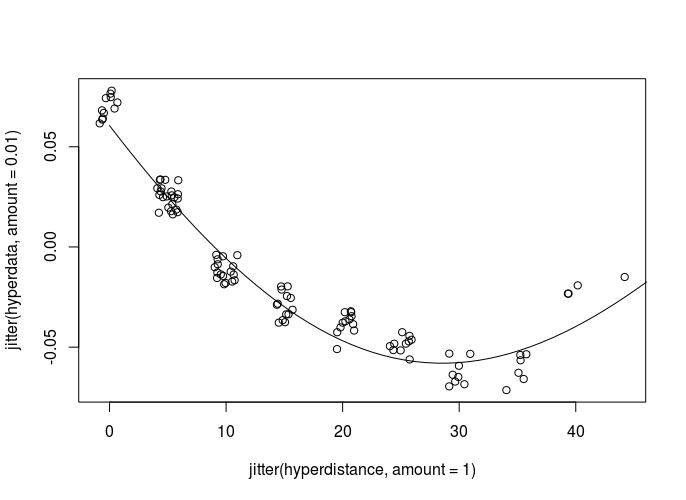
\includegraphics[scale=0.5]{PrezImage6.png}
		
	\end{frame}
	
	\begin{frame}
		\frametitle{Proposition 2: Use DS to Develop Priors for Parametric Kernel}
		
		Idea: 
		
		\begin{itemize}
			\item Fix some parametric form
			\item With loose priors, develop a posterior on DS with no nugget over train and test points.
			\item Use posterior as prior for real data analysis.
		\end{itemize}
		
		\vspace{1em}
		
		For this project: Moment-match IG prior
		
	\end{frame}
	
	\section[Section]{Simulations with Univariate Continuous Response.}
	
	\begin{frame}
		\frametitle{Problem setup}
		
		\begin{itemize}
			\item Release gas in a room. 
			\item Observe spread along 1 dimension at some points.
			\item Predict concentration at unobserved points.
		\end{itemize}
		
		The scientist's model:
		
		$$\frac{\partial S}{\partial t} = D \Delta$$
		
		$$\frac{\partial S}{\partial t} = D \frac{\partial^2 S}{\partial x^2}$$
		
		Observation:
		
		$$f_{obs} = f_{true} + \epsilon$$
		
		$$\epsilon \sim N(0,0.1)$$
		
	\end{frame}
	
	\begin{frame}
		\frametitle{Sim 1: Setup}
		
		\begin{itemize}
			\item The scientists model is perfect.
		\end{itemize}
		
		Scientist's Model:
		
		$$\frac{\partial S}{\partial t} = 10 \frac{\partial^2 S}{\partial x^2}$$
		
		Boundary conditions of zero, initial condition of mass throughout space.
		\vspace{1em}
		
		Truth:
		
		$$\frac{\partial S}{\partial t} = 10 \frac{\partial^2 S}{\partial x^2}$$
		
	\end{frame}
	
	\begin{frame}
		\frametitle{Sim 1: DiffEQ Solution}
		
		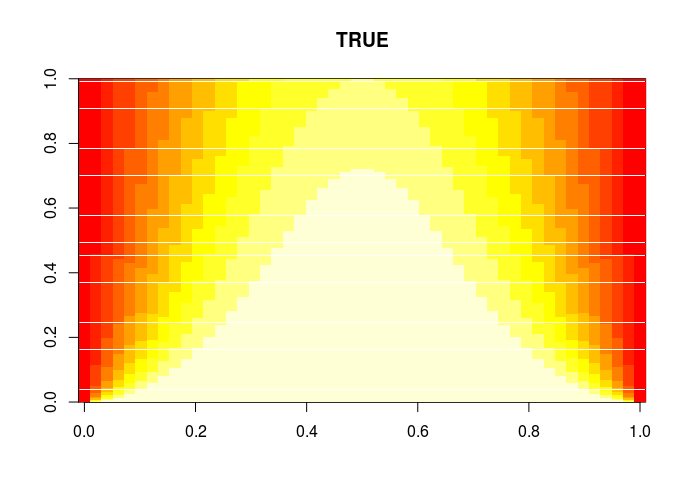
\includegraphics[scale=0.65]{PrezImage7.png}
		
	\end{frame}
	
	\begin{frame}
		\frametitle{Sim 1: Results}
		
		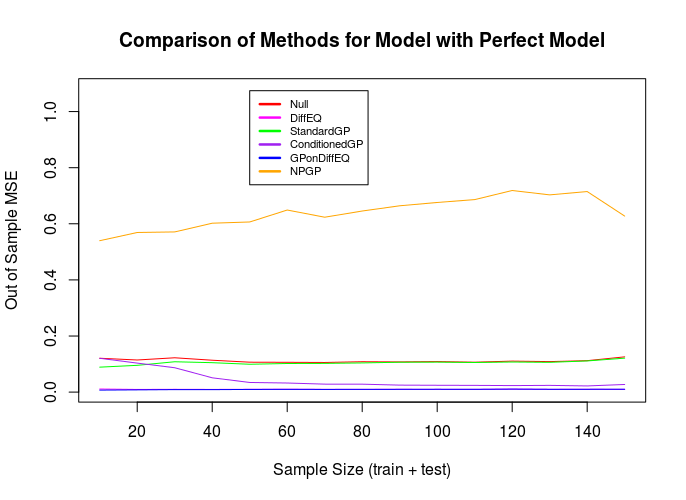
\includegraphics[scale=0.5]{PrezImage4.png}
		
	\end{frame}
	
	\begin{frame}
		\frametitle{Sim 1: Results}
		
		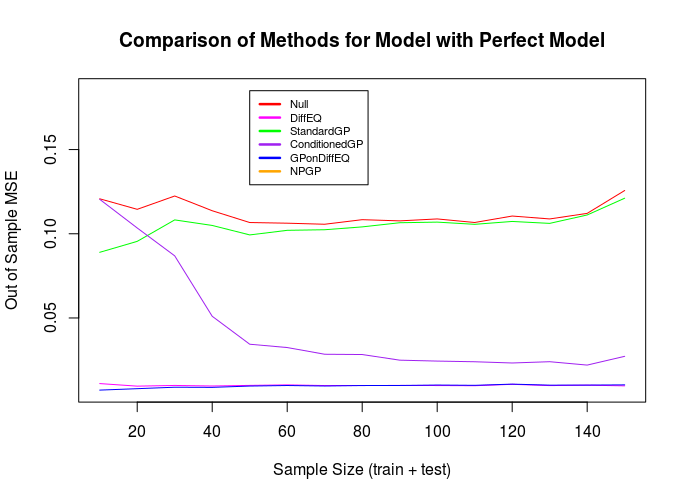
\includegraphics[scale=0.5]{PrezImage5.png}
		
	\end{frame}
	
	\begin{frame}
		\frametitle{Sim 3: Setup}
		
		\begin{itemize}
			\item The scientists model has the right parameter but the wrong structure.
		\end{itemize}
		
		Scientist's Model:
		
		$$\frac{\partial S}{\partial t} = 10 \frac{\partial^2 S}{\partial x^2}$$
		
		Same boundary conditions
		\vspace{1em}
		
		Truth:
		
		$$\frac{\partial S}{\partial t} = 10 \frac{\partial^2 S}{\partial x^2} - 0.05 S R$$
		
		$$\frac{\partial R}{\partial t} = 10 \frac{\partial^2 R}{\partial x^2} - 0.05 S R$$
		
		Correct boundary conditions for S, R has initial mass 5 everywhere.
		
	\end{frame}
	
	\begin{frame}
		\frametitle{Sim 2: DiffEQ Solution}
		
		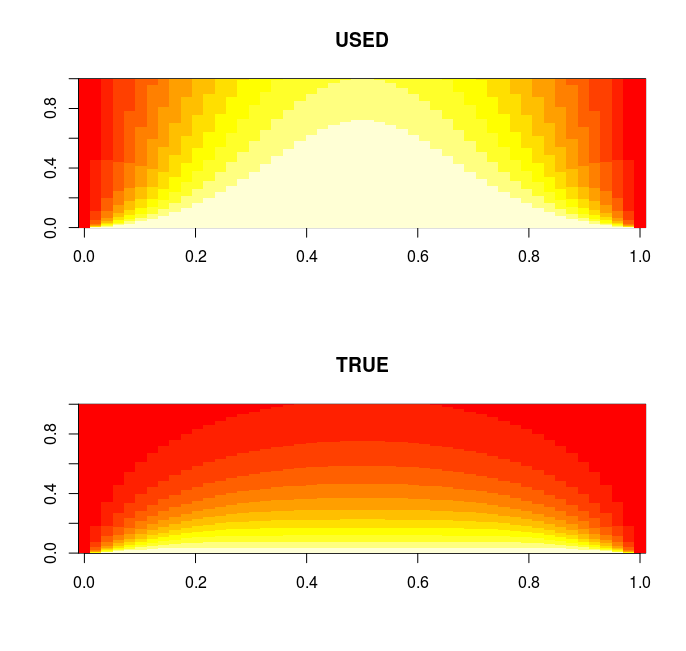
\includegraphics[scale=0.5]{PrezImage9.png}
		
	\end{frame}
	
	\begin{frame}
		\frametitle{Sim 2: Results}
		
		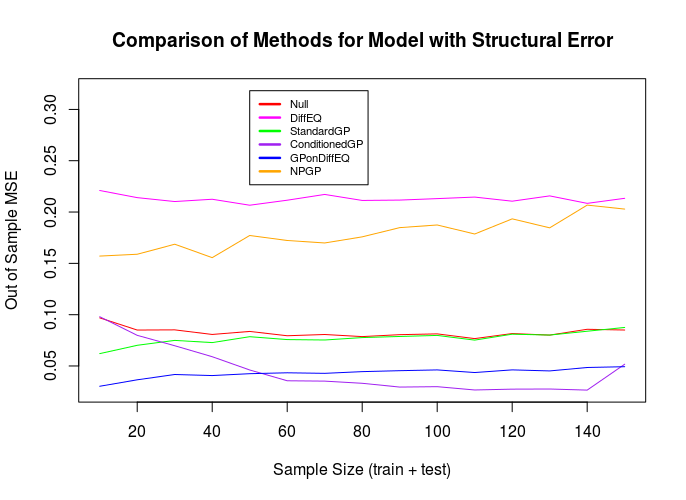
\includegraphics[scale=0.5]{PrezImage1.png}
		
	\end{frame}
	
	\begin{frame}
		\frametitle{Future Work}
		
		Kernels in between:
		
		\begin{itemize}
			\item The NP kernel seems to adapt too much to the hyperdata, not enough to real data.
			\item Conditioned kernel may not bond to hyperdata enough.
			\item Can they be merged somehow?
		\end{itemize}
		
		Fit GP without integration:
		
		$$cov(f_i, \frac{\partial f_i}{\partial x_{dj}}) = \frac{\partial k(x_i, x_j)}{\partial x_{dj}}$$
		
		Bayes-Hermite Integration.
		
	\end{frame}
\end{document}